\label{resultats}

\section{Exploration du corpus Charcot : \textsc{OBVIE} et \textsc{TextPair}}
Une première exploration du corpus Charcot à travers l'application OBVIE nous a permis d'identifier les substantifs les plus importants de chaque corpus en utilisant les fréquences brutes ou des méthodes plus fines comme \textsc{TF-IDF}, \textsc{BM25}, \textsc{$\chi$2} ou le \textsc{Test Gamma}. Cependant, l'application ne permet pas de quantifier la pertinence des expressions polylexicales (notamment les n-grammes de mots), très fréquentes dans les deux corpus et dont la décomposition entraînerait une perte d'information (p. ex. le terme polysémique \og{}bulbe\fg{} qui a une valeur spécifique dans l'expression figée \textit{bulbe rachidien}, \textit{cf}. fig. \ref{fig:bulbe}.
\begin{figure}[!h]
    \centering
    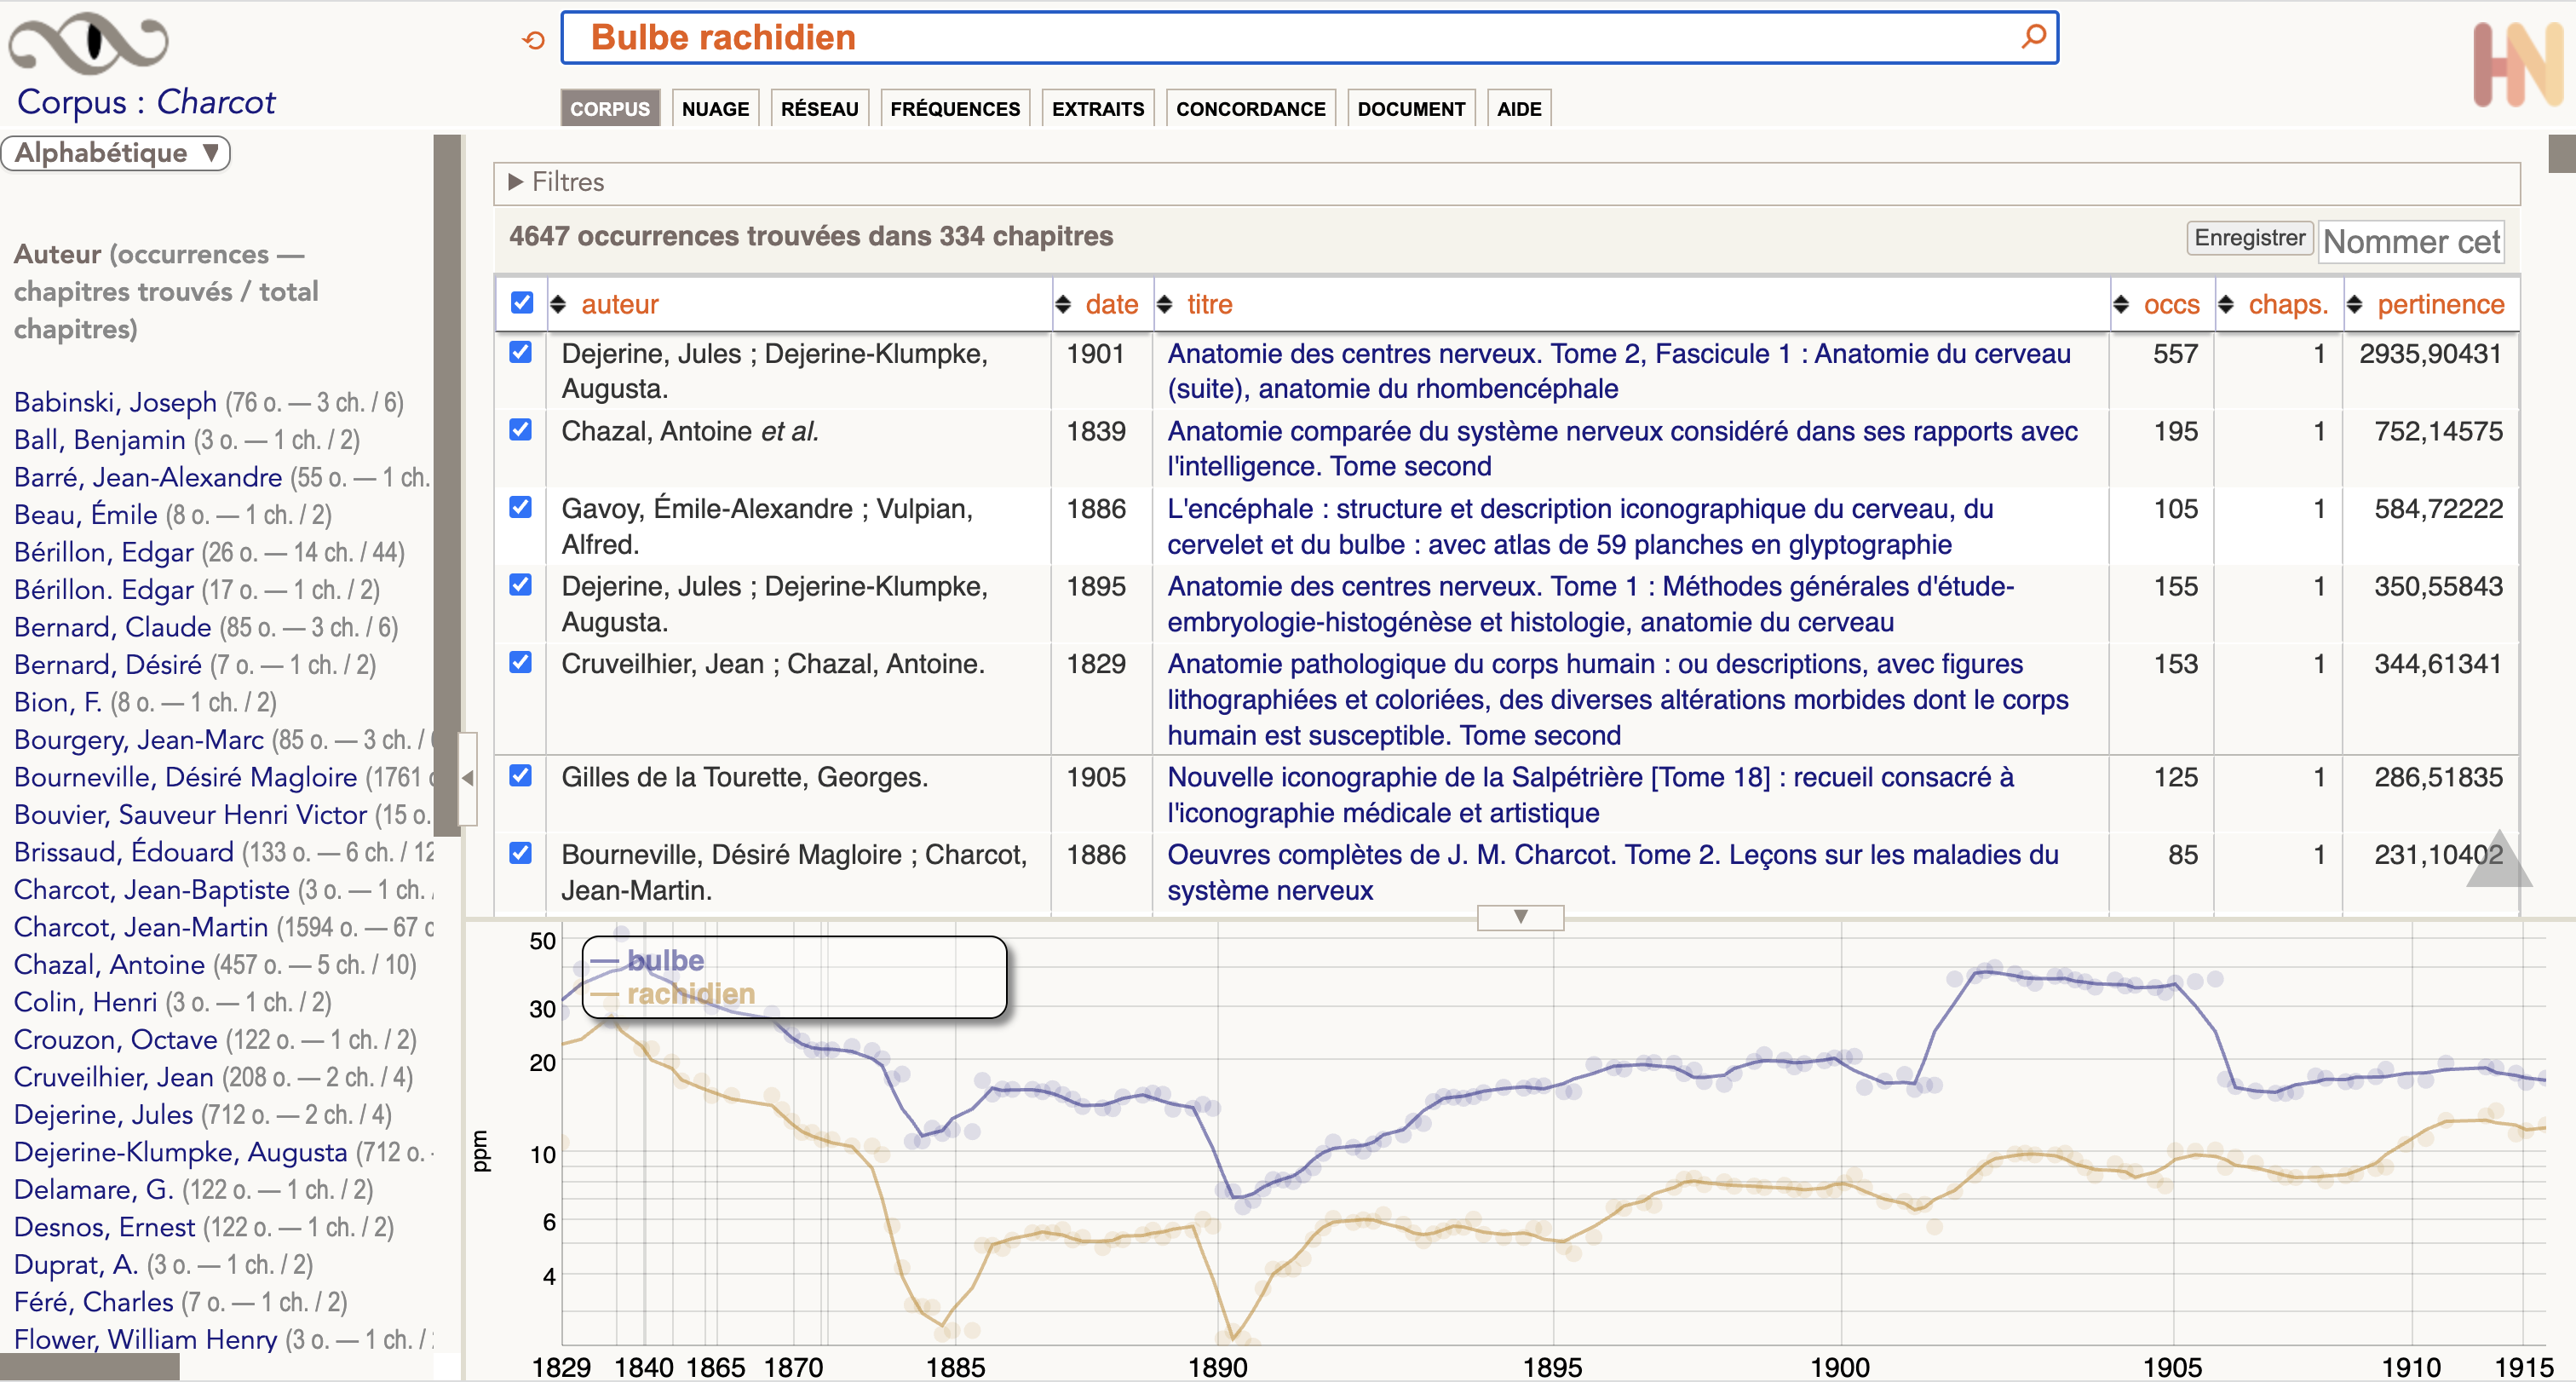
\includegraphics[width=1\textwidth]{img/bulbe_rachidien_mini.png}
    \caption{Distribution des fréquences des tokens avec la frise chronologique pour ceux constituant l'expression \textit{bulbe rachidien} (issus du corpus \og{}Charcot\fg{} et du corpus \og{}Autres\fg{}) dans le logiciel OBVIE. 
    % Pour raison de visibilité, l'image originale a été agrandie, ce qui a entraîné le rapprochement des années sur l'axe de l'abscisse.
    }
    \label{fig:bulbe}
\end{figure}

Concernant l'alignement des séquences similaires aux deux corpus, \textsc{TextPair} nous a permis, par une lecture attentive, de faire des comparaisons entre les textes et de rechercher des termes au sein des passages similaires, malgré le nombre de résultats assez conséquent (\textit{cf}. la figure \ref{fig:textpair}).

\begin{figure}[!h]
    \centering
    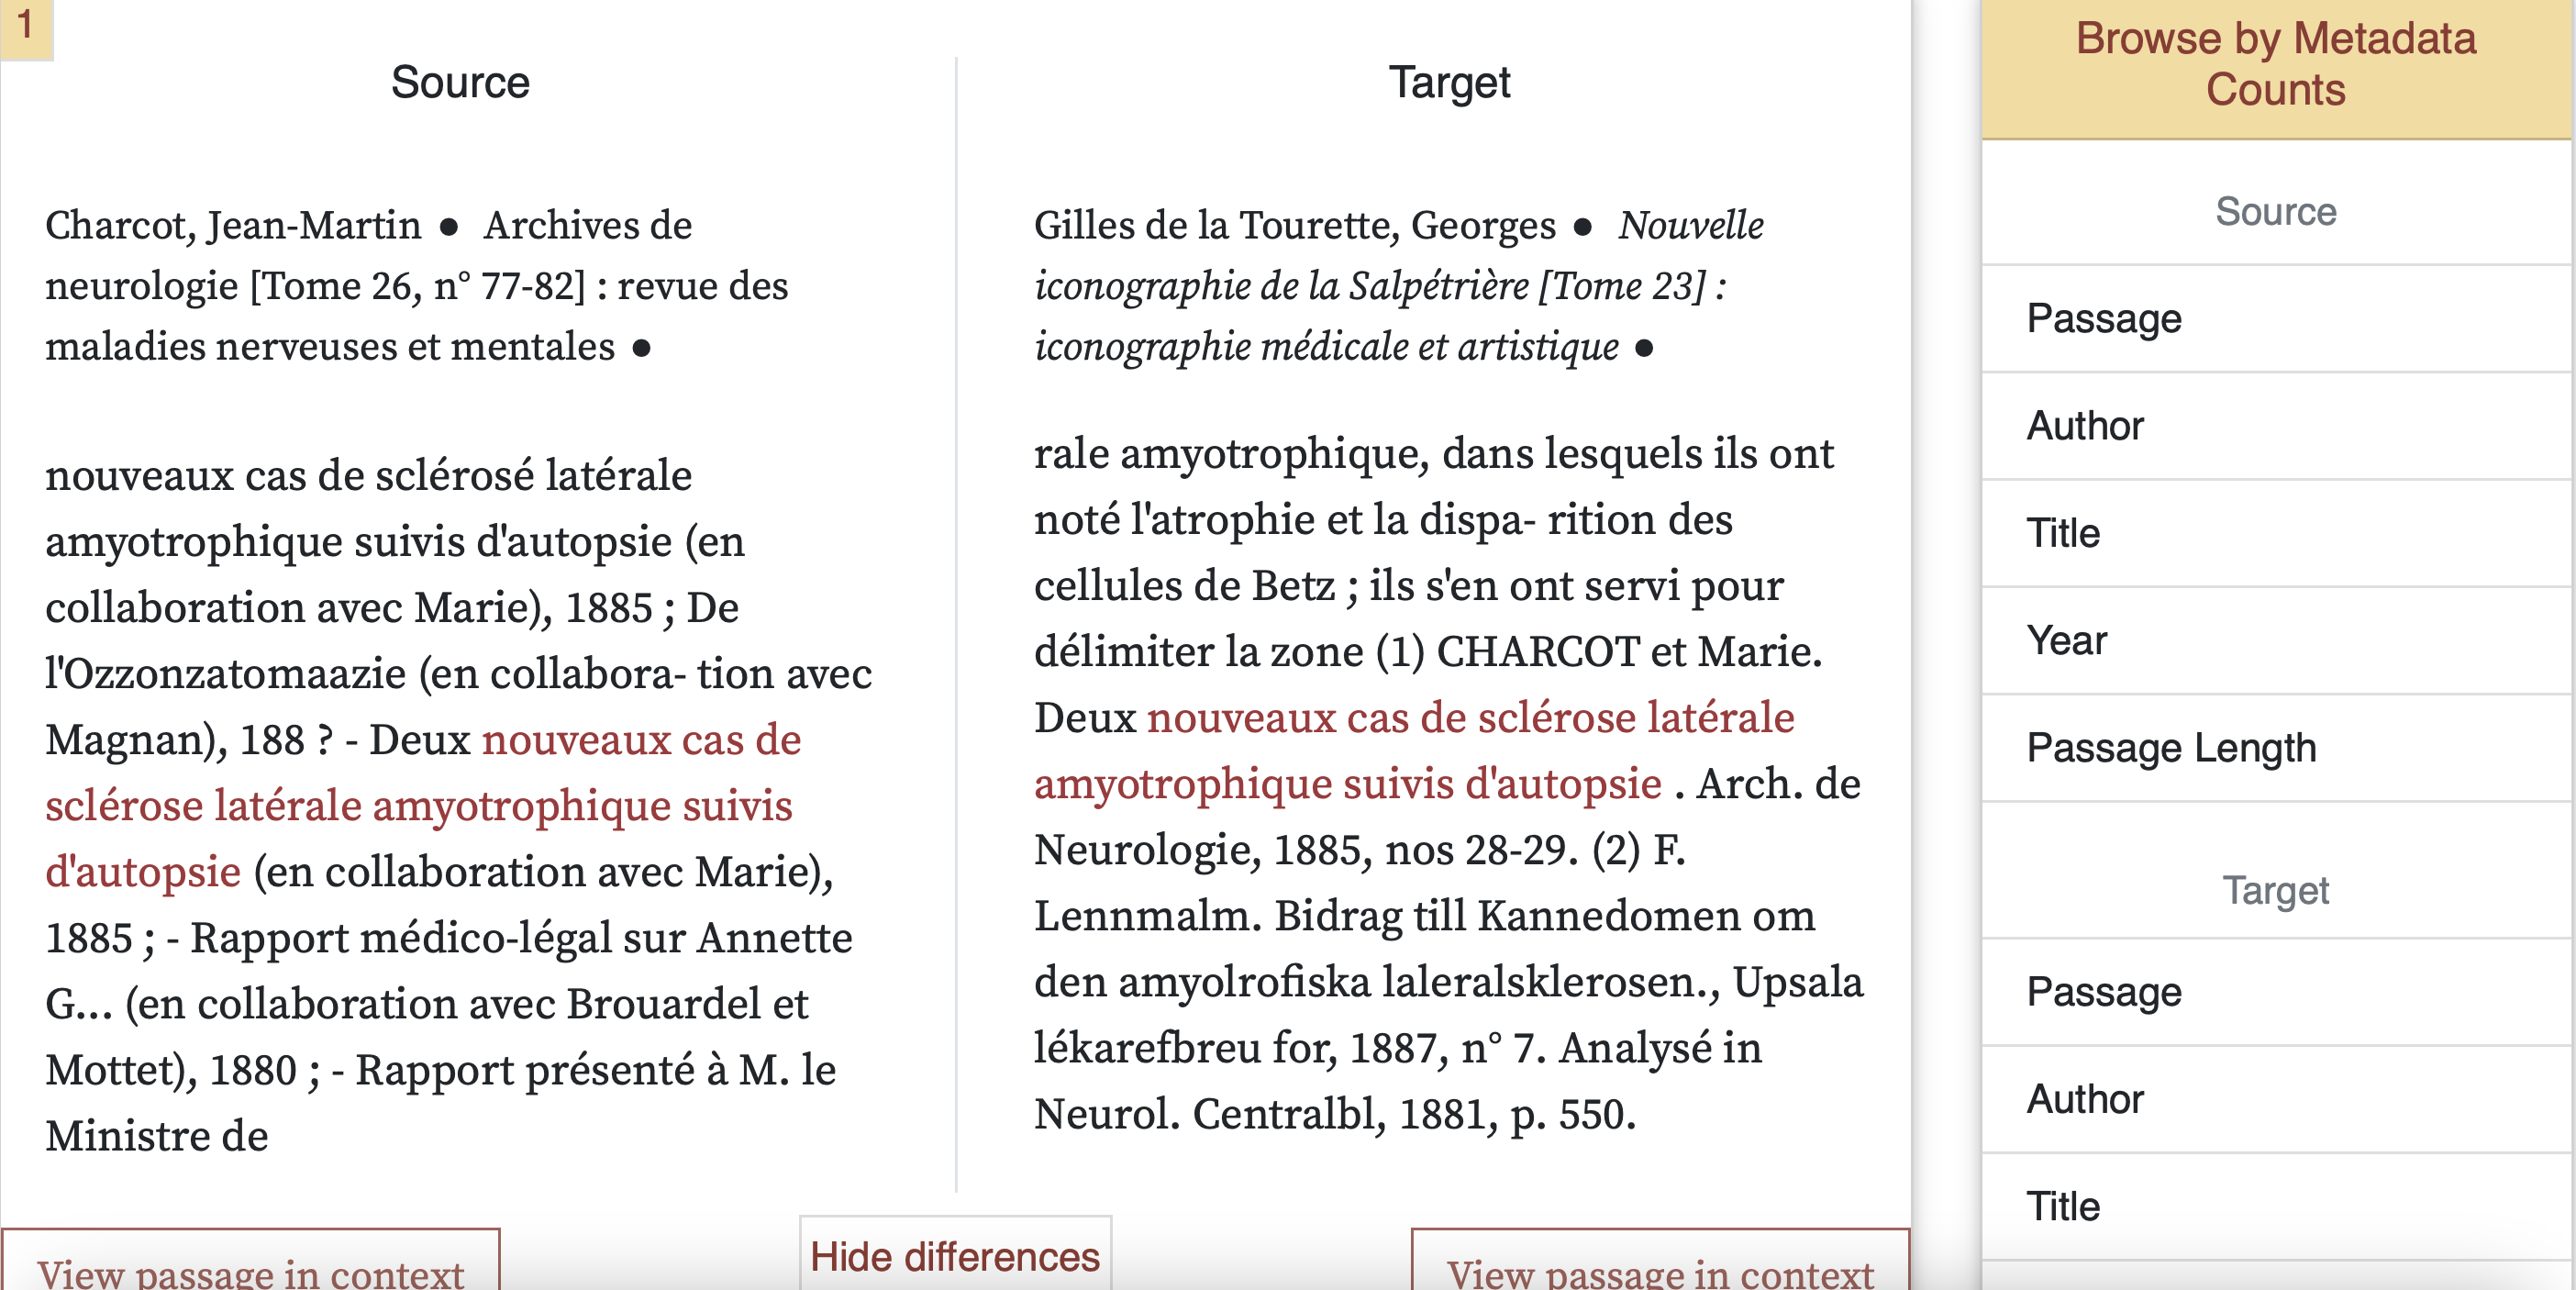
\includegraphics[width=1\textwidth]{img/textpair.png}
    \caption{Alignement et comparaison des textes de Charcot à celui de Georges Gilles de la Tourette (le seul résultat) en lançant la requête \textit{sclérose latérale amyotrophique}.}
    \label{fig:textpair}
\end{figure}
\section{Extraction des phrases-clés : méthode statistique}
\section{Extraction des phrases-clés : méthode à base d'apprentissage profond}
\section{Discussion}
